\documentclass[tikz]{standalone} %\usetikzlibrary{calc} 
%\usepackage{rubikcube,rubikrotation,rubikpatterns,rubiktwocube} 
\usepackage{pgfopts}
\usepackage{graphicx}
\usepackage{xcolor}
\usepackage{tikz}
\usetikzlibrary{3d,arrows.meta}
%\newcommand{\CycleThreeEdgesFlipTwo}{[CycleThreeEdgesFlipTwo],F,R,U,Rp,Up,Fp}%
%\newcommand{\cyclethreeedgesfliptwo}{\CycleThreeEdgesFlipTwo}%
\standaloneconfig{border=0bp}
%
%----corner sequences--------------------------
%\newcommand{\AllYellow}{[allyellow],R,U,Rp,U,R,Up,Up,Rp}% = SUNE  %cross -->allyellow
%\newcommand{\allyellow}{\AllYellow}%
%\newcommand{\CycleThreeCorners}{[cyclethreecorners],Lp,U,R,Up,L,U,Rp,Up}%
%\newcommand{\cyclethreecorners}{\CycleThreeCorners}%
%\newcommand{\CornerRotation}{[CornerRotation],Up,Rp,Dp,R,U,Rp,D,R}
%\newcommand{\cornerrotate}{[cornerrotate],Up,Rp,Dp,R,U,Rp,D,R}
%\newcommand{\SwapTwoCorners}{[swaptwocorners],Rp,F,Rp,B2,R,Fp,Rp,B2,R2,Up}
%\newcommand{\swaptwocorners}{\SwapTwoCorners}
%\newcommand{\CornerOrientation}{[CornerOrientation],Rp,D2,R,Bp,U2,B,Rp,D2,R,Bp,U2,B} % (R^{-1} D^2 R B^{-1} U^2 B)^2
%\newcommand{\EdgeOrientation}{[EdgeOrientation],Sr,U,Sr,U,Sr,U2,Srp,U,Srp,U,Srp,U2}
%
%% brace and bracket macros 
%\newcommand{\Rubikbracket}[1]{$\left(\mbox{#1}\right)$}
%\newcommand{\Rubikbrace}[1]{$\left\{\mbox{#1}\right\}$}
%\newcommand{\cubenumber}[1]{\strut\raisebox{1cm}{#1}}
\definecolor{ptblue}{HTML}{2A5EA4}
\definecolor{surfblue}{HTML}{508ac3}
\definecolor{deepblue}{HTML}{243F57}
\definecolor{ash}{HTML}{CBD4C2}
\definecolor{pink-lavender}{HTML}{E0BAD7}
\definecolor{camel}{HTML}{C59F61}
\definecolor{dkgreen}{rgb}{0,0.6,0}
\definecolor{gray}{rgb}{0.5,0.5,0.5}
\definecolor{mauve}{rgb}{0.58,0,0.82}
\definecolor{remgrey}{RGB}{179,179,179}
\begin{document}
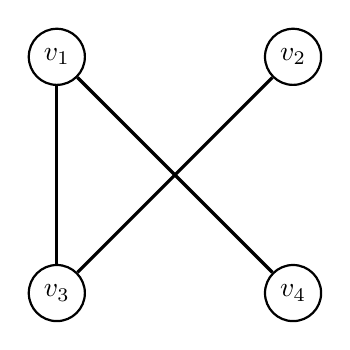
\begin{tikzpicture}
\begin{scope}[every node/.style={circle,thick,draw}]
    \node (A) at (0,3) {$v_1$};
    \node (B) at (3,3) {$v_2$};
%    \node (C) at (6,3) {$x_3$};
    \node (D) at (0,0) {$v_3$};
    \node (E) at (3,0) {$v_4$};
%    \node (F) at (4.5,0) {$x_6$} ;
% \node (G) at (7.5,0) {$x_7$} ;
\end{scope}
\begin{scope}[>={Stealth[black]},
              every node/.style={fill=white,circle},
              every edge/.style={draw=black,very thick}]
    \path [-] (A) edge  (D);
    \path [-] (A) edge (E);
%    \path [-] (A) edge (F);
%    \path [-] (A) edge (G);
    \path [-] (B) edge (D);
%    \path [-] (B) edge (F);
%    \path [-] (B) edge (G);
%    \path [-] (C) edge (F);
%    \path [-] (C) edge (E); 
%    \path [-] (C) edge  (G); 
\end{scope}
\end{tikzpicture}
\end{document}